\section{Problem description}\label{sec:problem-descr}
% Prompt: State objectives and specifications of the lab being solved in your own words.
This project uses a STM32F0 Discovery microcontroller (hereafter referred to as ``the microcontroller'') and a PBMCUSLK project board (``the project board'') to both generate and monitor a pulse width modulated (PWM) signal.
A potentiometer on the project board controls a signal voltage that is read by the analog-to-digital (ADC) converter on the microcontroller.
Using the ADC voltage, the microcontroller calculates the potentiometer resistance value and generates an output voltage via digital-to-analog (DAC) conversion.
The output signal is isolated with a 4N35 optocoupler and used to control the frequency of a NE555 timer.
The square wave timer output is fed back into the microcontroller, which measures the timer output signal frequency.
The microcontroller uses its serial peripheral interface (SPI) to pass data to an LCD on the project board.
The timer frequency and potentiometer resistance are displayed on the LCD and updated on an ongoing basis.
Figure~\ref{fig:systemblocks} shows the interactions of the major system components.

\begin{figure}[tbph]
  \centering
  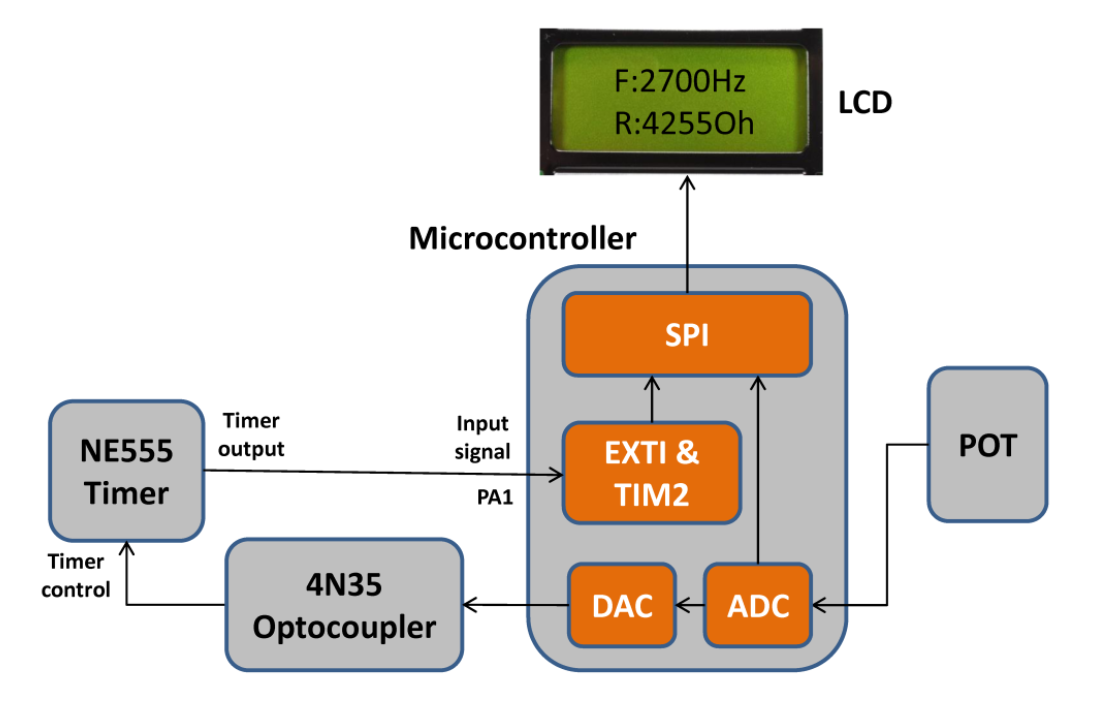
\includegraphics[width=0.7\linewidth]{../graphics/system_blocks}
  \caption{Block diagram for microcontroller-based resistance and frequency measurement system~\cite{lab-manual}}
  \label{fig:systemblocks}
\end{figure}

The lab manual~\cite{lab-manual} specifies some constraints on development, for pedagogical purposes:
\begin{itemize}
  \item Potentiometer voltage values must be obtained through polling,
  \item STM CMSIS functions are to be avoided; except,
  \item CMSIS may be used for SPI initialization and control.
\end{itemize}
